\documentclass[11pt,a4paper]{article}

% -------------------------------------------------
% PACKAGES
% -------------------------------------------------
\usepackage[utf8]{inputenc}
\usepackage[T1]{fontenc}
\usepackage[english]{babel}

\usepackage{geometry}
\geometry{left=2.5cm,right=2.5cm,top=2.5cm,bottom=2.5cm}

\usepackage{graphicx}
\usepackage{float}
\usepackage{hyperref}
\usepackage{booktabs}
\usepackage{longtable}
\usepackage{enumitem}
\usepackage{xcolor}
\usepackage{caption}
\usepackage{geometry}
\geometry{left=1.7cm,right=1.7cm,top=1.8cm,bottom=1.8cm}

\usepackage{listings}
\lstset{
  basicstyle=\ttfamily\small,
  breaklines=true,
  frame=single,
  numbers=left,
  numberstyle=\tiny,
  keywordstyle=\color{blue},
  commentstyle=\color{gray},
  stringstyle=\color{teal},
  showstringspaces=false
}

% -------------------------------------------------
% DOCUMENT INFO
% -------------------------------------------------
\title{\textbf{HandGestures2Bot} \\ Project Documentation}
\author{HandGestures2Bot \\ Mobile Embedded and Development / Hochschule Aalen}
\date{\today}

% -------------------------------------------------
% BEGIN DOCUMENT
% -------------------------------------------------
\begin{document}

\maketitle
\thispagestyle{empty}
\vspace{1cm}

\begin{center}
\textbf{Repository:} \href{https://github.com/notWetro/HandGestures2Bot.git}{HandGestures2Bot on GitHub}
\end{center}

\newpage
\tableofcontents
\newpage

% =================================================
% 1. PROJECT OVERVIEW AND GOAL
% =================================================
\section{Project Overview and Goal}
HandGestures2Bot is a project that enables controlling a TurtleBot robot using hand gestures captured or voice  via a mobile application.
The main goal is to provide an intuitive and modern way of robot control without traditional controllers, by using gesture recognition and network communication.

\subsection{Goal of the Project}
The main objectives of this project are:
\begin{itemize}[leftmargin=1.5cm]
    \item Provide a gesture-based robot control mechanism.
    \item Provide a voice-based robot control mechanism.
    \item Enable an easy setup process for connecting the robot and the mobile app.
    \item Ensure the system works reliably in a real environment (WiFi + Bluetooth provisioning).
    \item Keep the interaction focused on user experience and usability.
\end{itemize}

\subsection{Context Diagram / System Boundary}
This project connects a Flutter mobile app (gesture + voice control) with a TurtleBot3 running ROS~2.
The app sends movement commands via WebSocket over Wi-Fi. On the robot side, a safety scanner filters
the commands using LiDAR data and publishes safe velocity commands to the robot motors.
A Bluetooth provisioning service is used to configure the robot Wi-Fi and send the robot IP address back to the app.

\begin{figure}[H]
	\centering
	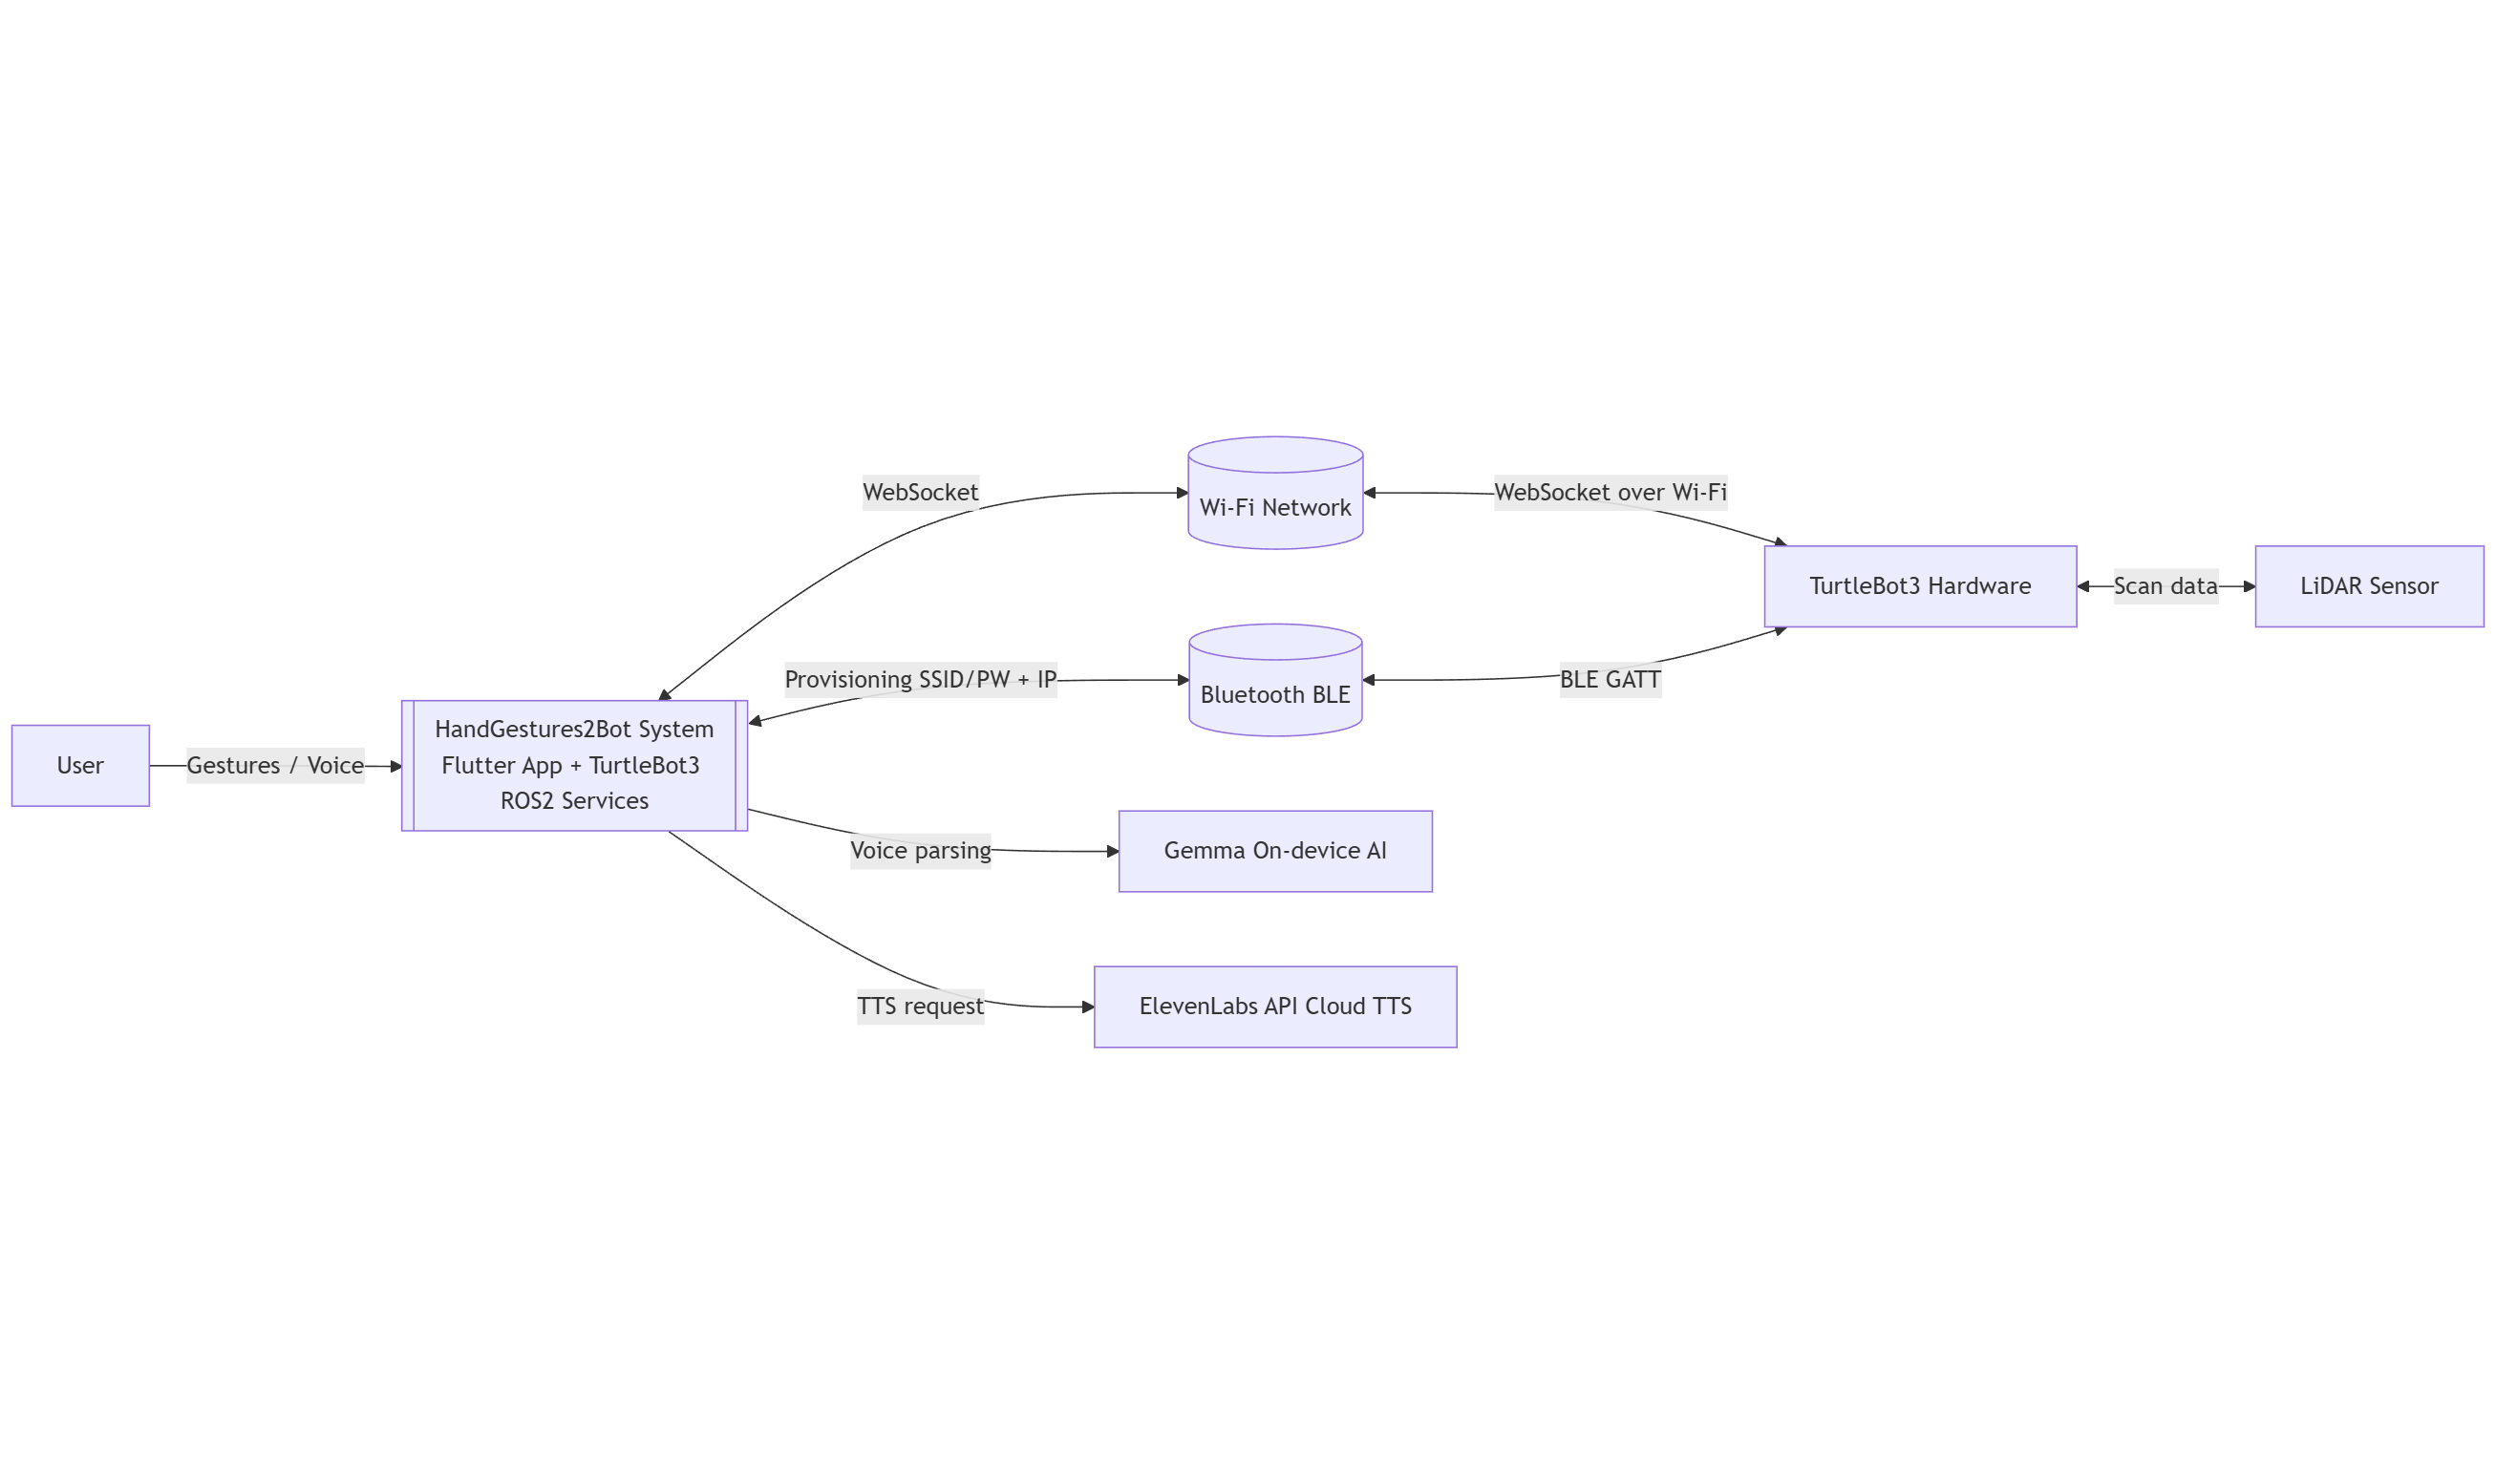
\includegraphics[width=1\textwidth]{figures/context_diagram_placeholder.png}
	\caption{Context Diagram (System Boundary)}
\end{figure}



\newpage
\subsubsection{External actors / environment}
\begin{itemize}[leftmargin=1.5cm]
	\item User (gesture + voice interaction)
	\item Wi-Fi network (WebSocket communication)
	\item Bluetooth Low Energy (Wi-Fi provisioning)
	\item TurtleBot3 hardware (motors + sensors) / LiDAR sensor (obstacle detection)
	\item ElevenLabs API (cloud TTS) / On-device AI model for voice command parsing
\end{itemize}

\subsubsection{Main interactions:}
\begin{itemize}[leftmargin=1.5cm]
	\item User $\rightarrow$ Flutter App: controls robot via gestures/voice
	\item Flutter App $\rightarrow$ Robot: sends \texttt{\{"movement": "..."\}} via WebSocket
	\item Robot $\rightarrow$ Flutter App: sends obstacle status updates
	\item Flutter App $\leftrightarrow$ Robot (BLE): sends Wi-Fi credentials and receives robot IP
\end{itemize}



% =================================================
% 2. FEATURES AND CAPABILITIES
% =================================================

\section{Features and Capabilities}

This section provides a high-level overview of the main features implemented in the HandGestures2Bot project.
Detailed scenarios and interaction flows are described in the next section.

\begin{itemize}[leftmargin=1.5cm]

	\item \textbf{Hand-gesture based robot control (Android):}
	Real-time gesture recognition using the camera and MediaPipe.

	\item \textbf{Voice-based robot control:}
	Speech-to-text, AI command interpretation, and optional TTS feedback.

	\item \textbf{Real-time robot control via WebSocket over Wi-Fi:}
	Sends JSON movement commands to the TurtleBot (\texttt{ws://<robot-ip>:8765}).

	\item \textbf{Supported movement commands:}
	Forward, backward, left, right, stop (unknown commands fall back to stop).

	\item \textbf{Safety obstacle filtering using LiDAR:}
	Blocks unsafe forward motion and prevents collisions.

	\item \textbf{Live obstacle status feedback to the mobile app:}
	Obstacle status updates are streamed back via WebSocket.

	\item \textbf{Bluetooth Low Energy (BLE) Wi-Fi provisioning:}
	Sends SSID/password and receives the robot IP address for Wi-Fi control.

	\item \textbf{Dance sequences / multi-step routines:}
	Gestures can trigger predefined movement sequences.

\end{itemize}

\newpage
% =================================================
% 3. SCENARIO AND FUNCTIONALITY DESCRIPTION
% =================================================
\section{Scenario and Functionality Description}

This section describes how the system is used across the system boundary.
The focus is on interactions between user/app/robot/network and not on internal architecture.

\subsection{Scenario 1: User controls the TurtleBot with Hand Gestures}
\textbf{Goal:} The user moves the TurtleBot using hand gestures detected by the mobile device.

\textbf{Actors:} User, Mobile App, TurtleBot

\textbf{Basic Flow:}
\begin{enumerate}[leftmargin=1.5cm]
    \item User opens the mobile app.
    \item The app activates gesture recognition using the device camera.
    \item Detected gestures are translated into movement commands.
    \item Commands are sent to the TurtleBot via WiFi.
    \item The TurtleBot executes movement (e.g., forward, left, right, stop).
\end{enumerate}

\begin{figure}[H]
    \centering
    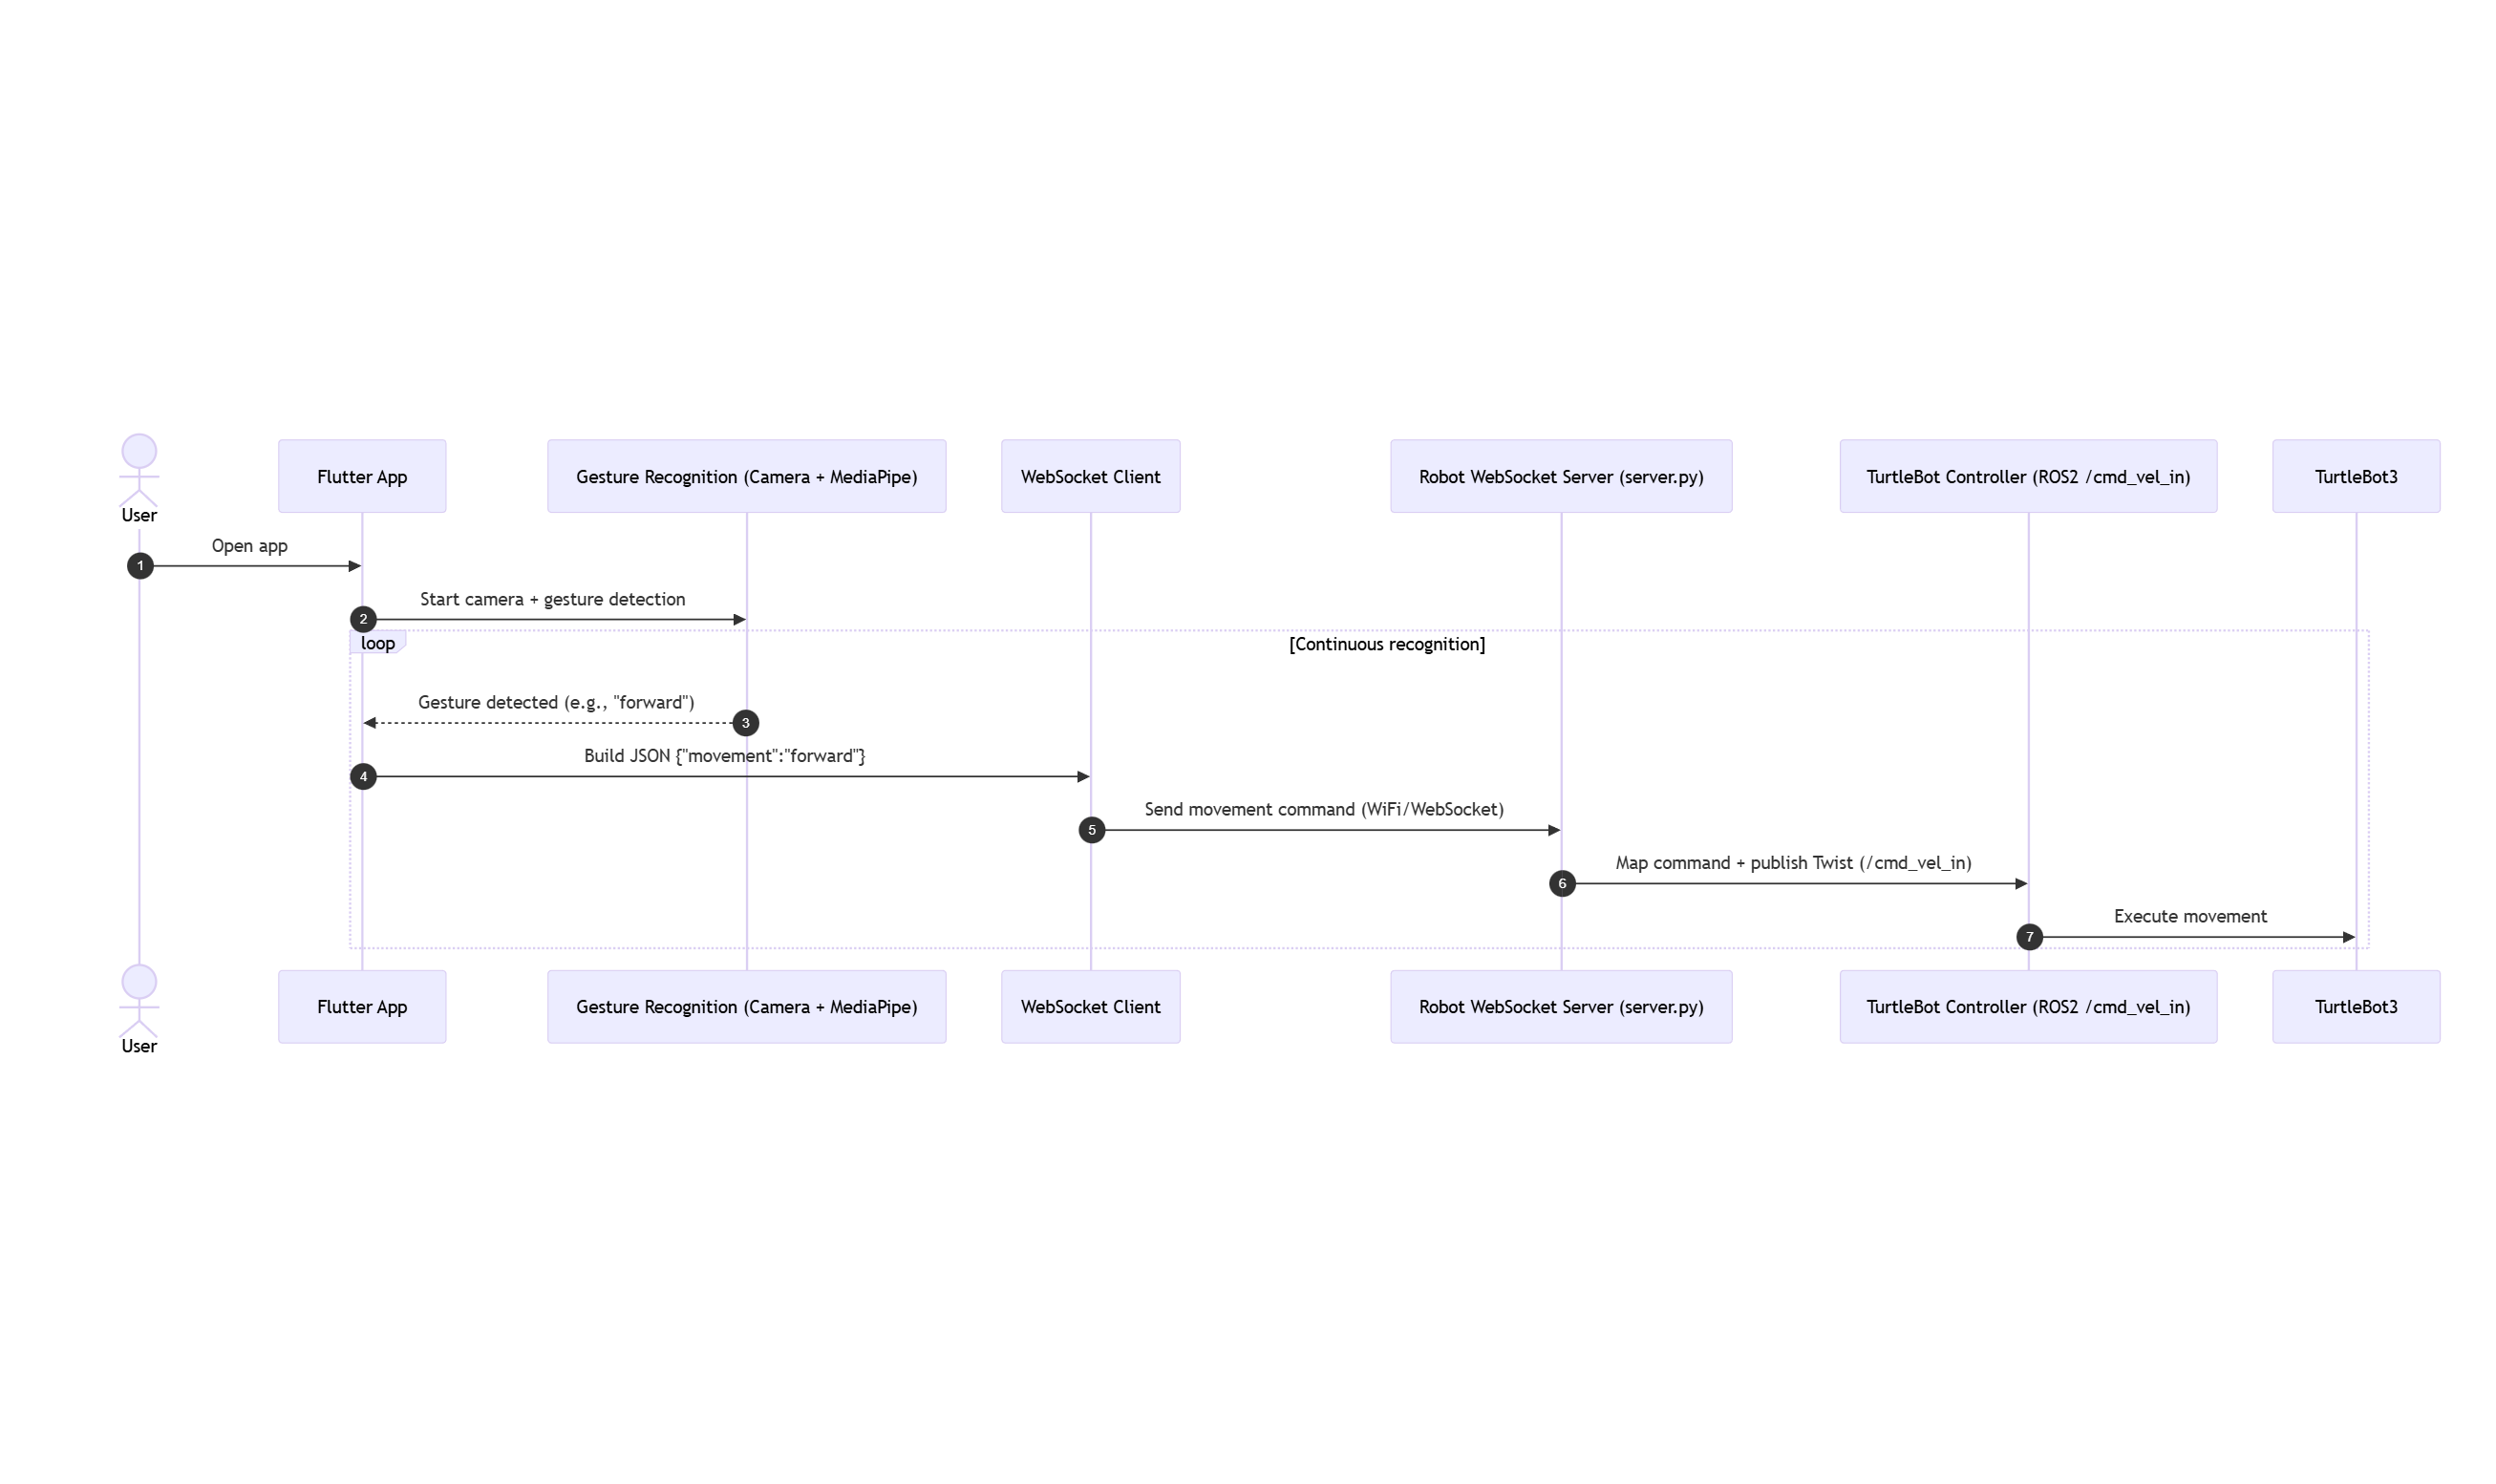
\includegraphics[width=1\textwidth]{figures/use_case_diagram_placeholder.png}
    \caption{Scenario 1 Sequence Diagram}
\end{figure}



\newpage
\subsection{Scenario 2: Bluetooth WiFi Setup (Provisioning)}
\textbf{Goal:} The user configures WiFi on the TurtleBot via Bluetooth, so that the app can connect via WiFi afterwards.

\textbf{Actors:} User, Mobile App, TurtleBot, Bluetooth, WiFi Network

\textbf{Basic Flow:}
\begin{enumerate}[leftmargin=1.5cm]
    \item User opens the Bluetooth WiFi Setup screen in the app.
    \item The app scans for nearby Bluetooth devices.
    \item The user selects the TurtleBot provisioning device.
    \item The app sends WiFi credentials (SSID + password).
    \item The TurtleBot connects to the WiFi network.
    \item The TurtleBot sends back connection status updates.
    \item The TurtleBot sends its assigned IP address to the app.
    \item The app saves the IP and switches to WiFi communication.
\end{enumerate}

\begin{figure}[H]
    \centering
    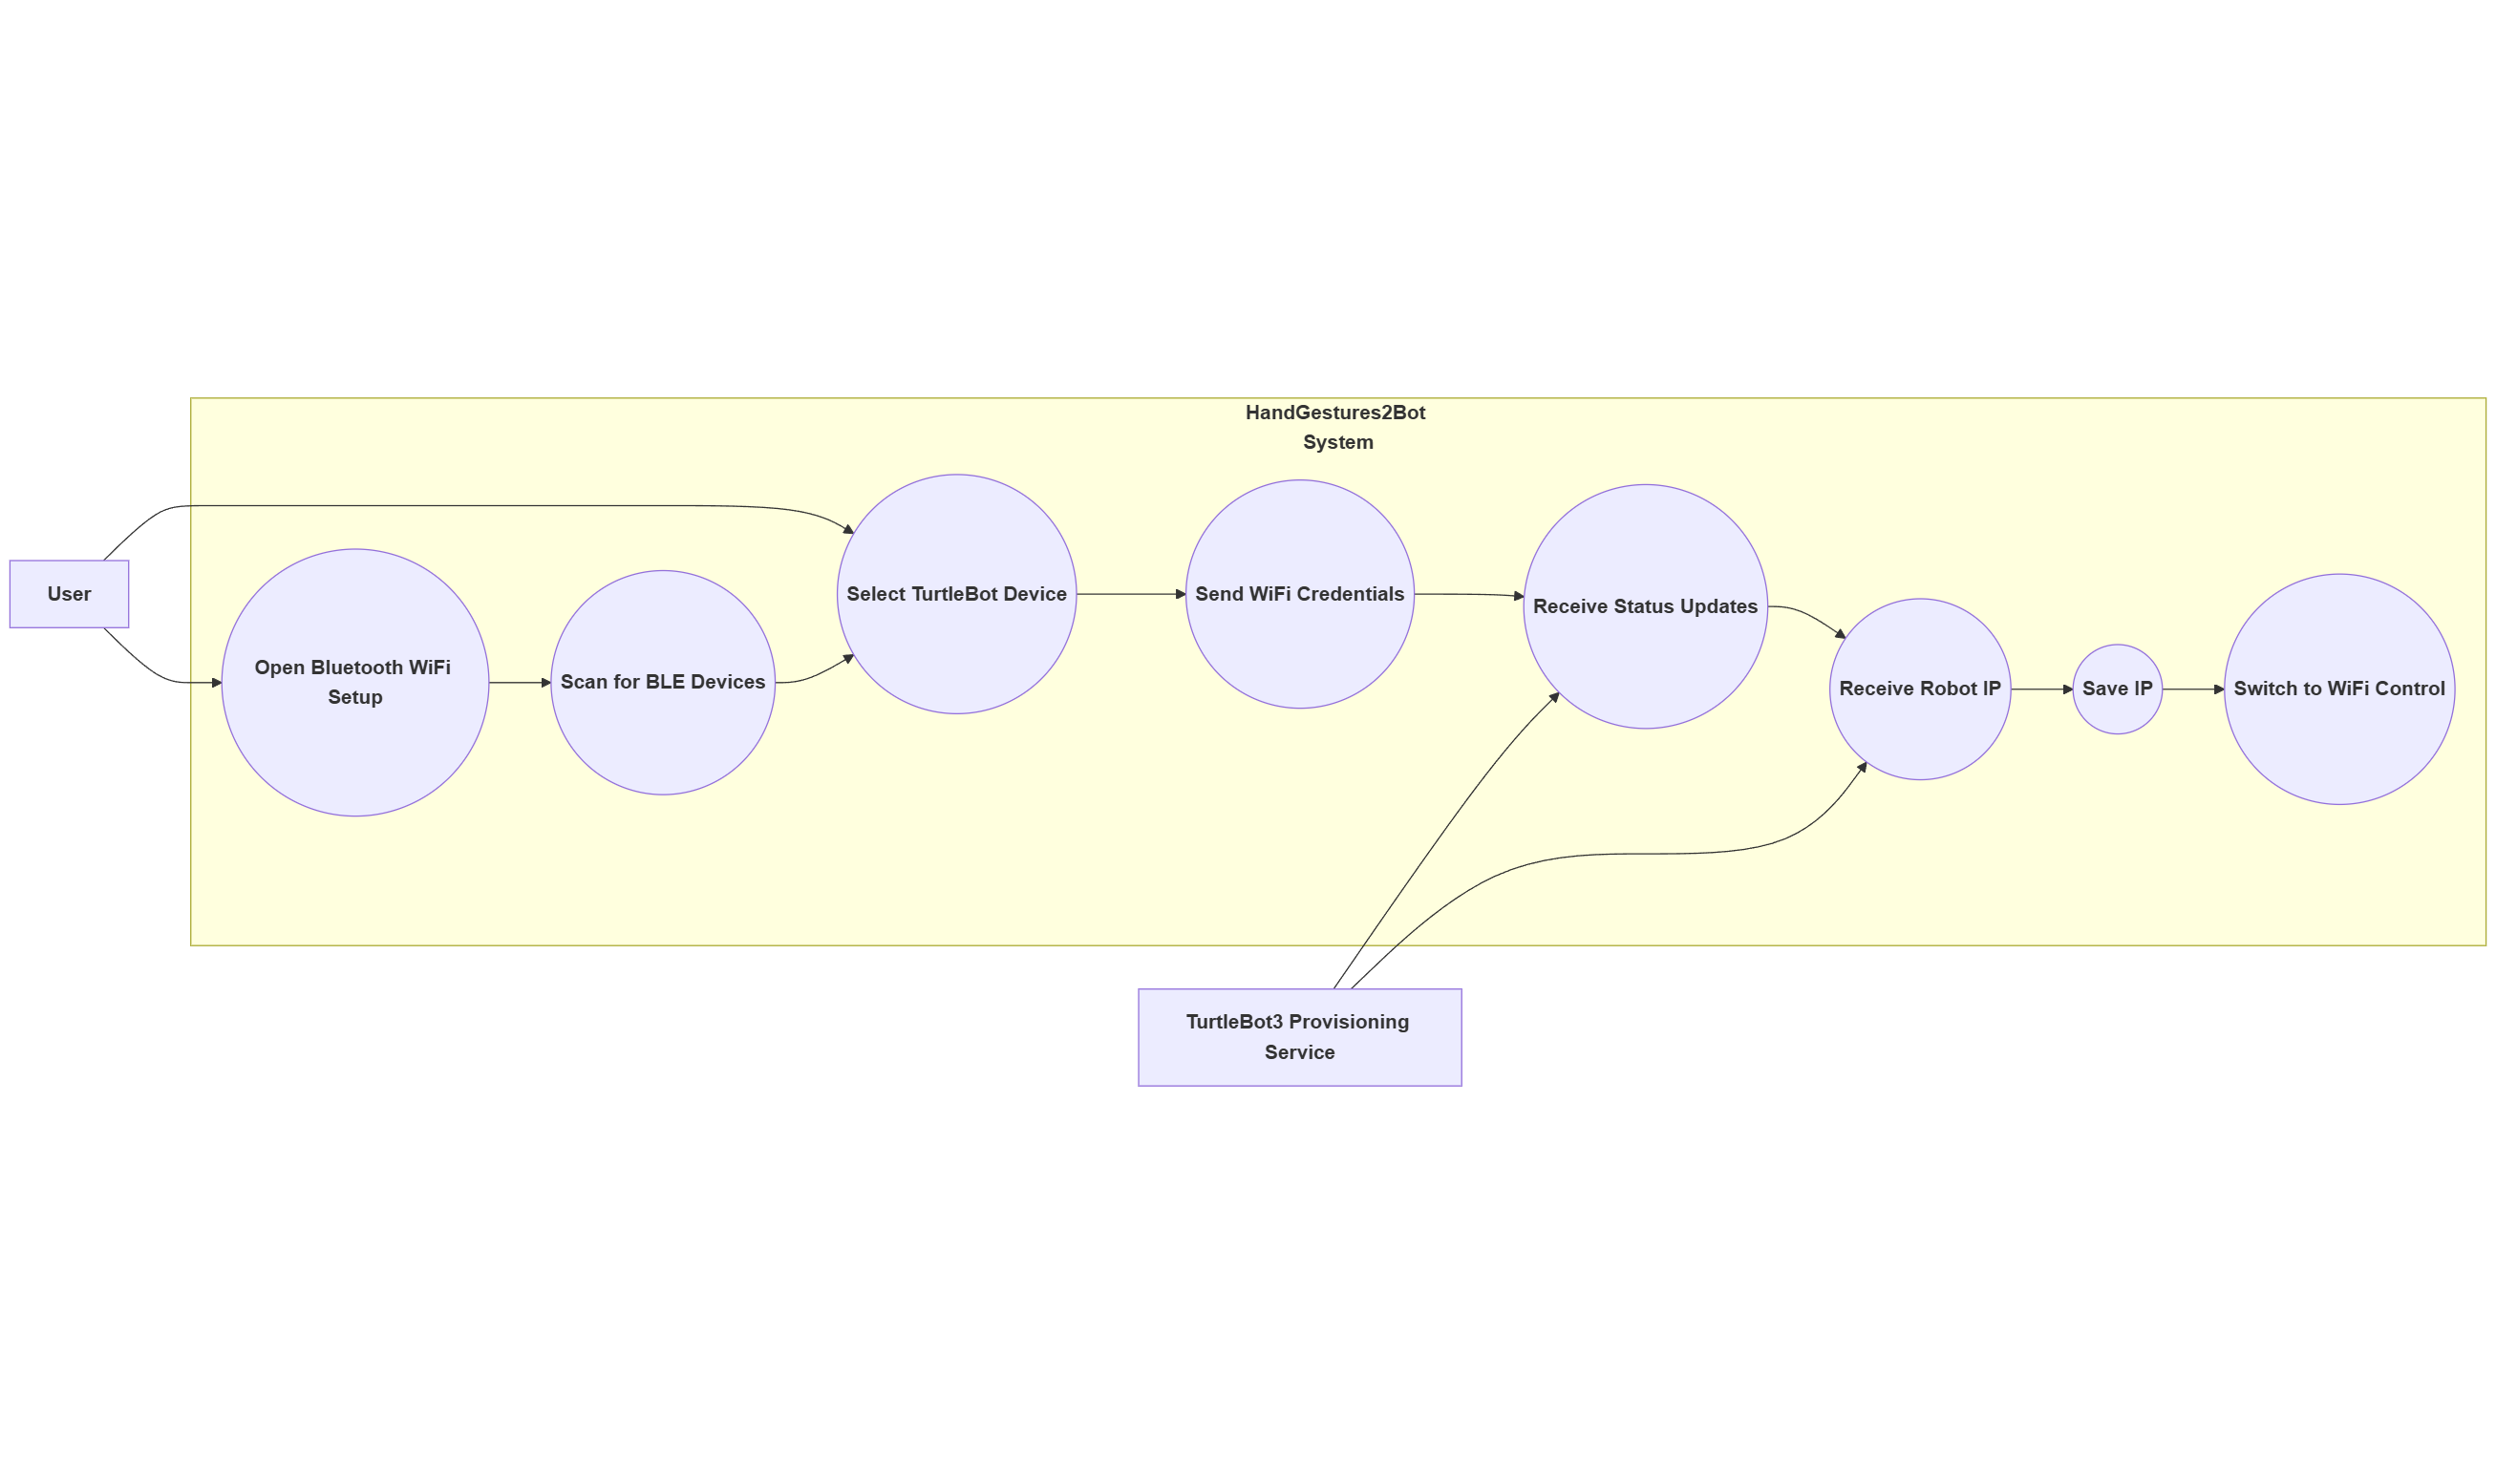
\includegraphics[width=0.95\textwidth]{figures/sequence_external_placeholder.png}
    \caption{Use Case Diagramm (App $\leftrightarrow$ Robot via Bluetooth/WiFi)}
\end{figure}



\newpage
\subsection{UI / Wireframes (No screenshots here)}
\begin{figure}[H]
    \centering
    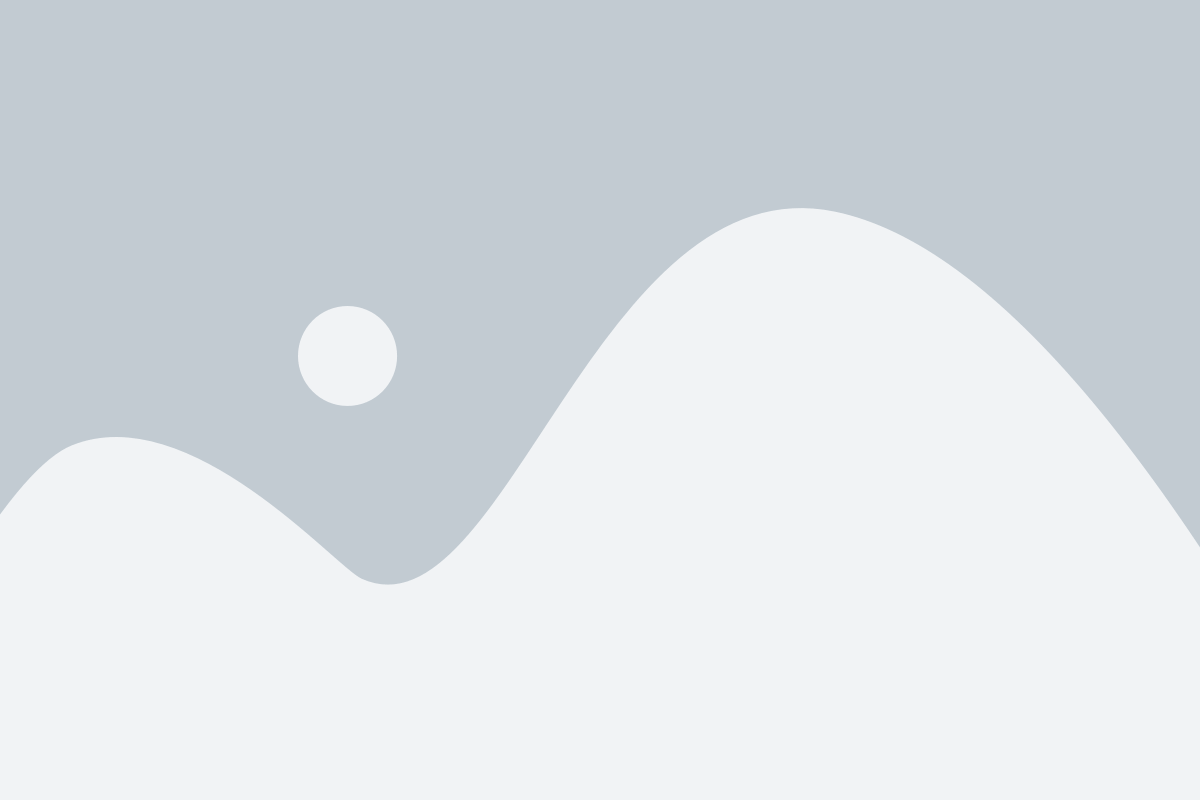
\includegraphics[width=0.9\textwidth]{figures/wireframe_placeholder.png}
    \caption{Wireframe Placeholder -- Bluetooth Setup and Gesture Control}
\end{figure}

% =================================================
% 4. ARCHITECTURE (INTERNAL)
% =================================================
\section{Architecture (Internal)}

This section describes the internal structure and interactions of the system.
It includes static and dynamic views of internal components.

\subsection{Static View (Components / Packages)}
The system consists of multiple major parts:

\begin{itemize}[leftmargin=1.5cm]
	\item \textbf{Flutter Mobile App (Dart):} Main user interface and control logic.
	\item \textbf{Gesture Recognition (MediaPipe):} Real-time hand tracking via native camera pipeline.
	\item \textbf{Voice Control:} Speech-to-text and AI-based command parsing.
	\item \textbf{Bluetooth Wi-Fi Provisioning (BLE):} Wi-Fi setup via Bluetooth Low Energy.
	\item \textbf{WebSocket Communication:} Robot control and status feedback over Wi-Fi.
	\item \textbf{Robot Control (ROS 2):} Velocity publishing and robot movement execution.
	\item \textbf{Safety Layer (LiDAR):} Obstacle detection and motion filtering.
\end{itemize}

\newpage
\subsection{Dynamic View (Key Internal Interactions)}
This section describes the most important runtime interactions between the main components of the system.

\subsubsection{Gesture Control $\rightarrow$ Robot Movement}
\textbf{Goal:} Move the TurtleBot using hand gestures from the mobile app.

\begin{enumerate}[leftmargin=1.5cm]
	\item The native camera pipeline detects a hand gesture (MediaPipe).
	\item The gesture is forwarded to the Flutter app via the gesture MethodChannel.
	\item The Flutter UI maps the gesture to a movement command (e.g., \texttt{forward}).
	\item The app sends a JSON command over WebSocket to the robot.
	\item The robot WebSocket server receives the message and forwards it to the movement handler.
	\item The robot publishes a velocity command to \texttt{/cmd\_vel\_in}.
	\item The safety scanner filters unsafe motion using LiDAR data and publishes safe velocity to \texttt{/cmd\_vel}.
\end{enumerate}

\subsubsection{Obstacle Feedback $\rightarrow$ App Warning Overlay}
\textbf{Goal:} Inform the user when motion is blocked due to obstacles.

\begin{enumerate}[leftmargin=1.5cm]
	\item The safety scanner reads LiDAR scan data from \texttt{/scan}.
	\item It computes obstacle distances and publishes an obstacle status message on \texttt{/obstacle\_status}.
	\item The robot WebSocket server subscribes to \texttt{/obstacle\_status} and broadcasts updates to connected clients.
	\item The mobile app receives the obstacle status via WebSocket.
	\item The UI overlays warnings and blocked-motion indicators in the camera view.
\end{enumerate}

\subsubsection{Bluetooth Wi-Fi Provisioning}
\textbf{Goal:} Configure robot Wi-Fi credentials and obtain the robot IP address.

\begin{enumerate}[leftmargin=1.5cm]
	\item The user opens the Bluetooth Wi-Fi Setup page in the app and starts scanning.
	\item The phone connects to the robot provisioning device via BLE.
	\item The app sends SSID and password to the robot via BLE characteristics.
	\item The robot connects to the Wi-Fi network and updates its provisioning status.
	\item The robot sends status updates and its assigned IP address back to the app.
	\item The app stores the IP locally and uses it for future WebSocket connections.
\end{enumerate}

\subsubsection{Voice Control $\rightarrow$ Robot Movement}
\textbf{Goal:} Move the robot using spoken commands.

\begin{enumerate}[leftmargin=1.5cm]
	\item The user speaks a command in the voice control view.
	\item The app converts speech to text (STT).
	\item The AI service  interprets the text and generates a movement command.
	\item The command is sent via WebSocket to the robot (same path as gesture control).
	\item Chosen ElevenLabs  opsion sends feedback to play the voice action.
\end{enumerate}


\begin{figure}[H]
	\centering
	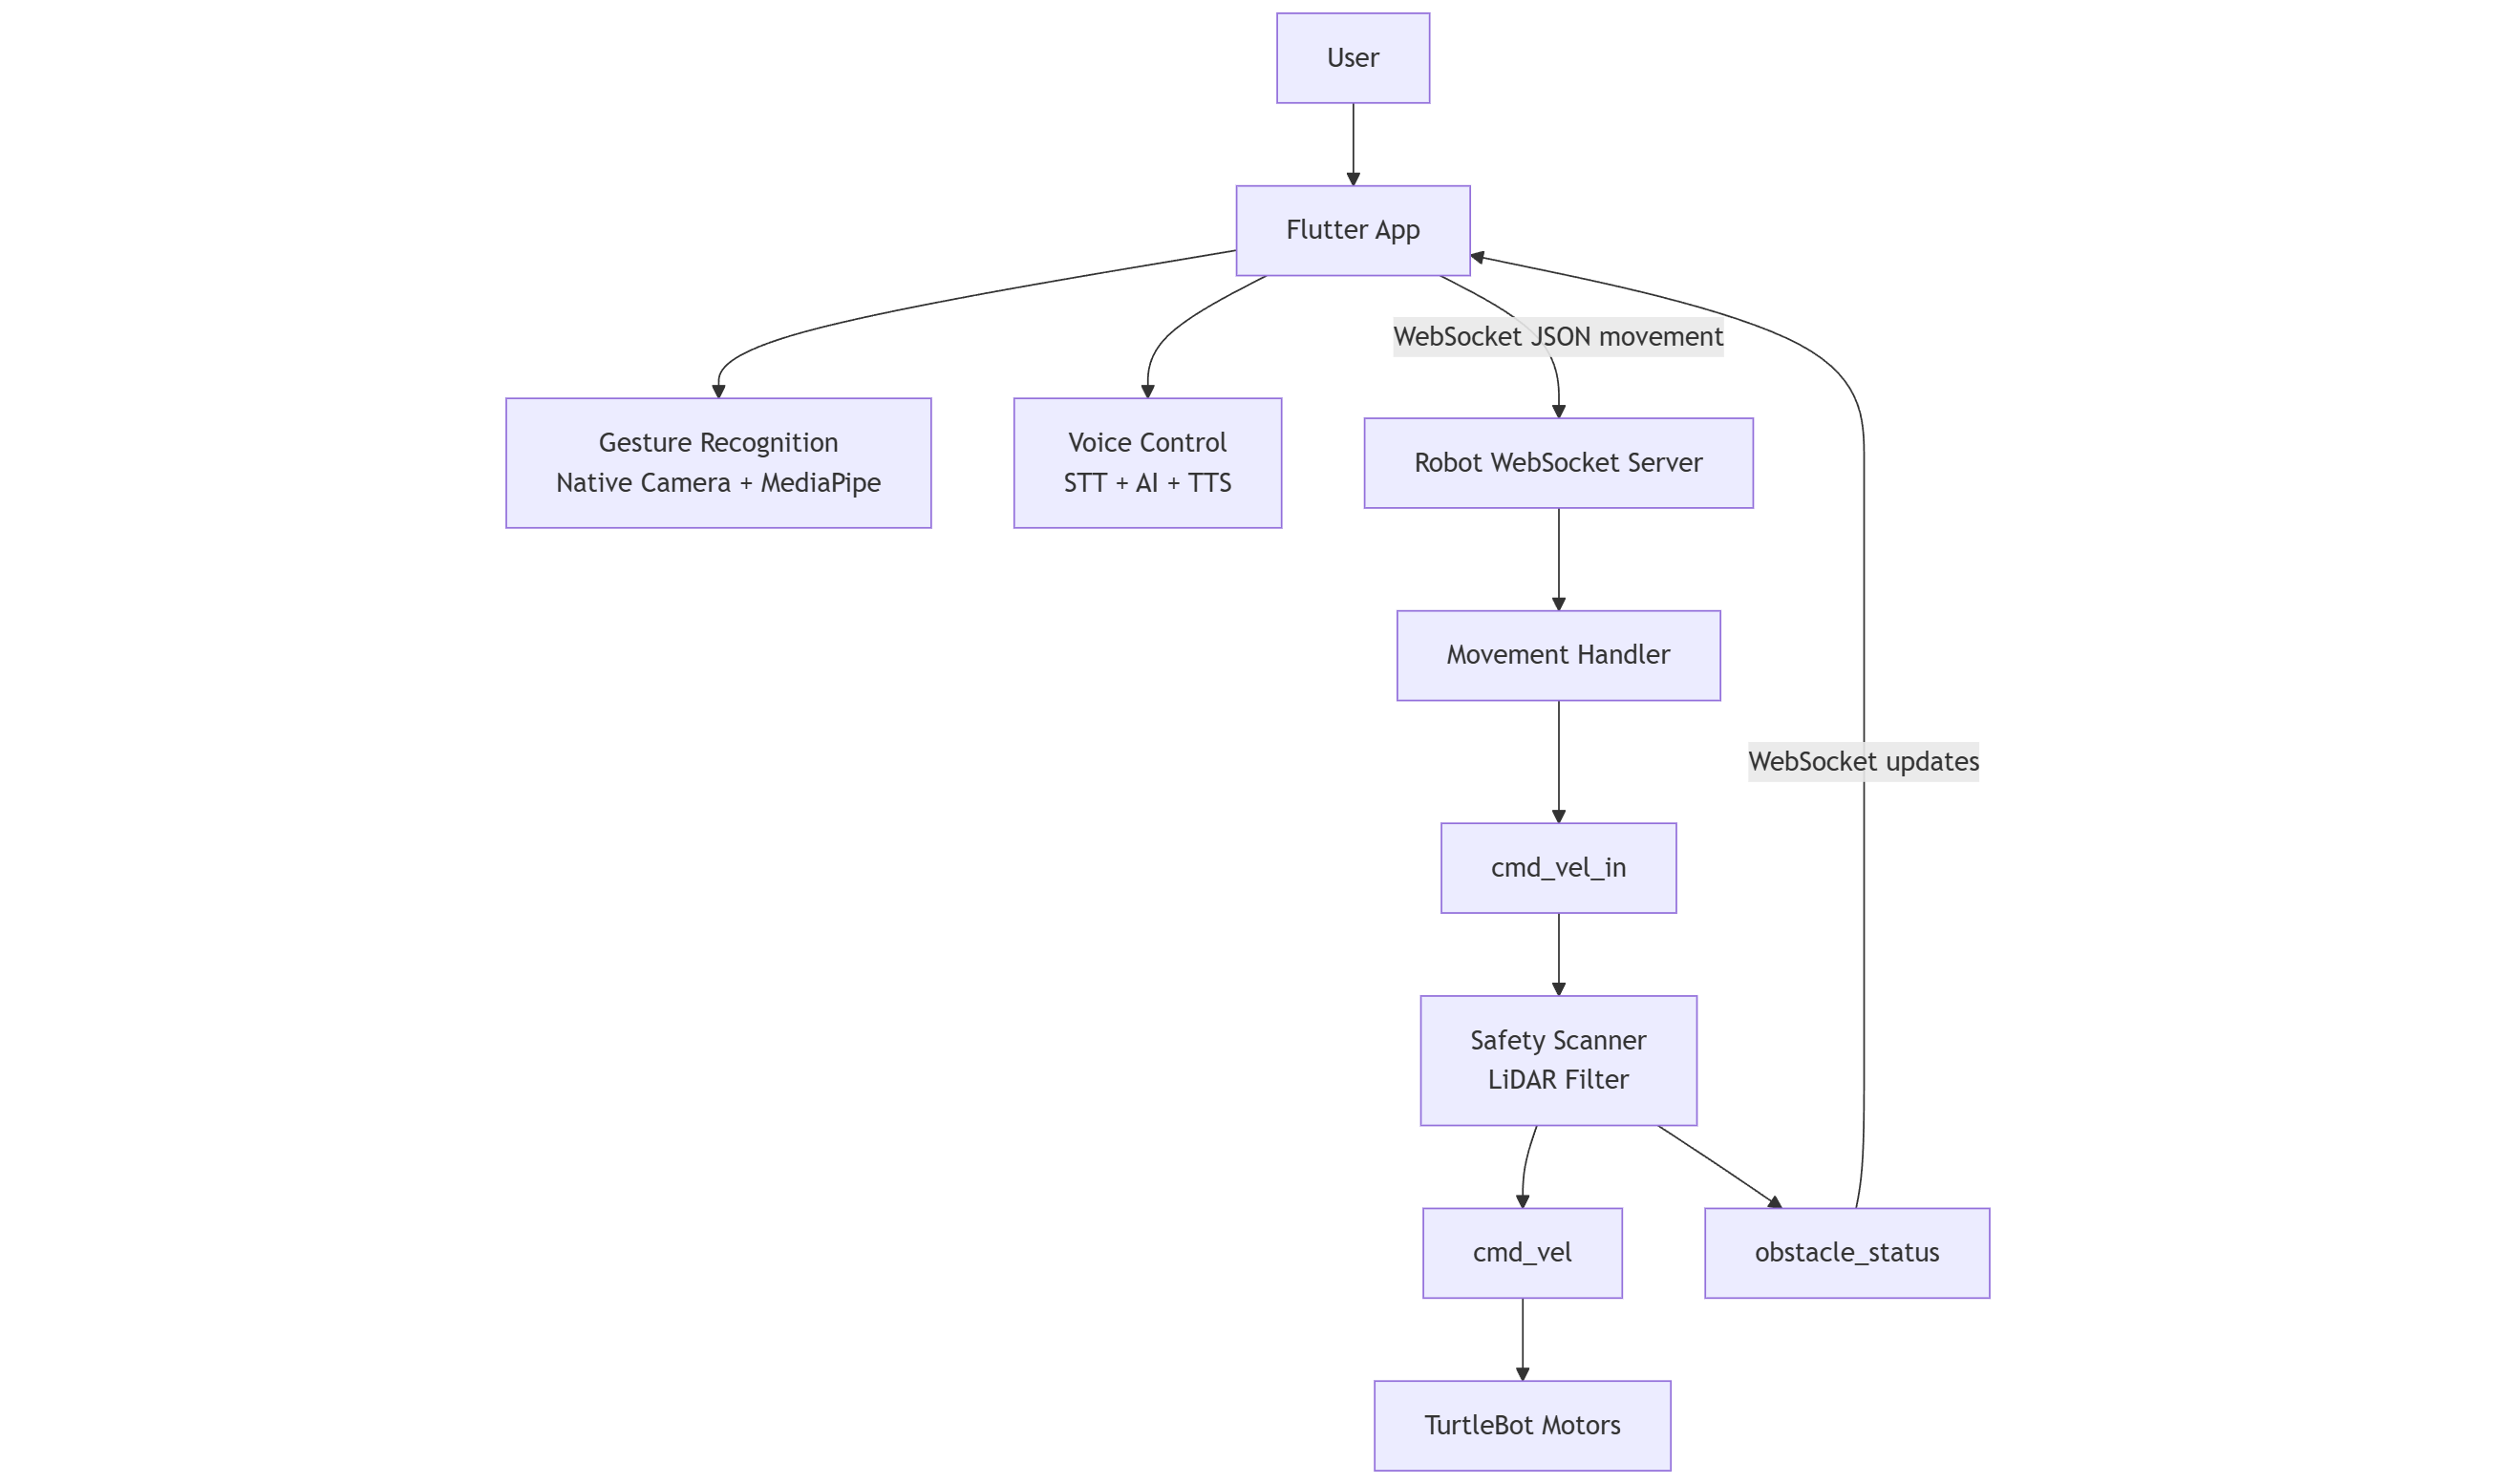
\includegraphics[width=0.9\textwidth]{figures/dynamic_view.png}
	\caption{Flowchart (Data Flow Diagram / System Interaction Flow)}
\end{figure}

% =================================================
% 5. TECHNOLOGIES AND REFERENCES
% =================================================

\newpage
\section{Technologies, Libraries, and References}

This section lists all important technologies, libraries, frameworks, and reused components.
This is necessary to avoid plagiarism assumptions.

\subsection{Technologies Used (excluding iOS)}
\begin{itemize}[leftmargin=1.5cm]
	\item Flutter SDK (Material UI) for the mobile application
	\item WebSocket communication over Wi-Fi for robot control
	\item Bluetooth Low Energy (BLE) for Wi-Fi provisioning
	\item Android CameraX for camera preview and analysis
	\item MediaPipe Tasks Vision for hand landmark detection and gesture recognition
	\item ROS 2 Humble for robot control and messaging
	\item TurtleBot3 platform (real robot and simulation)
\end{itemize}

\subsection{Important Libraries / Frameworks}
\begin{itemize}[leftmargin=1.5cm]
	\item \textbf{Flutter / Dart:} \texttt{web\_socket\_channel}, \texttt{shared\_preferences}, \texttt{speech\_to\_text},
	\texttt{flutter\_tts}, \texttt{http}, \texttt{audioplayers}, \texttt{flutter\_gemma}
	\item \textbf{Android:} CameraX, MediaPipe Tasks Vision, Android BLE GATT stack
	\item \textbf{Robot / ROS 2:} \texttt{rclpy}, standard ROS messages, Python \texttt{websockets}
	\item \textbf{Robot BLE provisioning:} BlueZ / \texttt{bluezero}, \texttt{netifaces}, \texttt{wpa\_cli} / \texttt{nmcli}
\end{itemize}

\subsection{External Services / Assets}
\begin{itemize}[leftmargin=1.5cm]
	\item ElevenLabs Text-to-Speech API (cloud service)
	\item MediaPipe hand landmark model file (\texttt{hand\_landmarker.task})
	\item GEMMA LLM ai Bot
\end{itemize}

\subsection{Reused / Preexisting Components}
\begin{itemize}[leftmargin=1.5cm]
	\item TurtleBot3 hardware platform and its base ROS ecosystem
	\item ROS 2 Humble and TurtleBot3 packages (e.g., bringup and Gazebo simulation)
	\item Preinstalled ROS 2 simulation packages on the provided Ubuntu virtual maschine from lab lecture (used for testing and simulation)
	\item MediaPipe framework and pretrained hand landmark model
	\item GEMMA LLM ai Bot
\end{itemize}


%NIKLAS TODO: Please start here if you have anything to add regarding iOS implementation
\subsection{Important Implementation Notes for iOS}

During the process, it has been decided that we will stop the development of the iOS app and
concentrate exclusively on the Android platform. This approach was necessitated by basic technological incompatibilities
between \textit{MediaPipe} and \textit{Gemma} on iOS.

Additionally, Gemma internally depends on \textit{MediaPipe Tasks} and hence comes bundled with preincluded native MediaPipe integration.
Specifically with regards to an iOS ecosystem, MediaPipe is very sensitive to multiple or parallel integrations
with native C++, Protobuf, and Swift modules. In our project, MediaPipe was already used for camera-based gesture recognition.
Introducing Gemma in addition to this existing setup resulted in severe linker- and module conflicts, manifesting in
unresolved native symbols and build-time errors.

Though a similar problem with Android could be addressed through selective omission of certain MediaPipe modules,
its counterpart is absent on iOS devices. A possible solution would have required replacing or extensively restructuring
the entire existing MediaPipe communication layer so that only the MediaPipe version bundled with Gemma remained in use.
This would have implied a fundamental change to the overall project architecture, particularly affecting the camera pipeline,
frame processing, and native iOS integration.

The required implementation and testing effort would have been disproportionate to the scope of the project and
would have introduced a significant risk of additional errors and development delays. For these reasons, the iOS app was dropped,
and development efforts were concentrated on Android, where the coexistence of MediaPipe and
Gemma can be implemented in a technically stable and reliable manner.

\subsection{Why we dropped dance moves via AI}

Since the LLM we are using is not advanced enough to reliably understand the complex prompts required to trigger dance moves via voice commands,
we decided not to implement this functionality.

The LLM started returning incorrect JSON files, which interfered with the core functionality of the voice control. Additionally, once a dance move was triggered,
it was often not cleared properly and continued to execute repeatedly, even when only a simple movement direction was given.

\section{Lessons Learned}

One of the key lessons learned during the project was the importance of thoroughly evaluating technology choices early on, especially when combining multiple frameworks or pipelines. In our case, the interaction between two frameworks led to unforeseen compatibility issues, particularly on the iOS platform. Future projects should include early feasibility studies or small proof-of-concept implementations to identify such risks in advance.

Another significant lesson was that developing a cross-platform application using Flutter is more complex than initially expected. While Flutter simplifies multi-platform development in theory, certain functionalities still required platform-specific (native) implementations. This resulted in duplicated effort and increased development time. The project highlighted that cross-platform solutions can introduce “unknown unknowns” that only emerge during implementation.

We also learned the importance of clearly defining required features and corresponding hardware dependencies at the beginning of the project. Some features were initially planned without fully understanding the hardware or system constraints they imposed. This led to design changes later in the development process, which could have been avoided with more detailed upfront planning.

A related lesson emerged from the integration of AI functionality. The application was originally designed to operate without an internet connection by relying on local processing. However, later decisions—such as integrating the ElevenLabs API—reintroduced the requirement for internet connectivity. This demonstrated the need to carefully evaluate architectural decisions and their long-term implications before implementation.

Additionally, the project emphasized the value of iterative testing and early integration. Several issues only became apparent once different system components were combined. Continuous integration and incremental testing would help detect such problems earlier in future projects.

Finally, from a team perspective, we learned the importance of clear communication and documentation. Regular alignment on technical decisions and explicit documentation of assumptions helped reduce misunderstandings and improved collaboration throughout the project.
\newpage
\section{Evaluation}

Table~\ref{tab:evaluation} summarizes the extent to which the implemented features achieved their intended objectives based on manual testing.

\begin{table}[h]
	\centering
	\caption{Evaluation of Implemented Features}
	\label{tab:evaluation}
	\begin{tabular}{|p{4.5cm}|p{6cm}|p{3cm}|}
		\hline
		\textbf{Feature / Functionality} & \textbf{Objective} & \textbf{Degree of Achievement} \\
		\hline
		Hand Gesture Recognition with Editing & Enable reliable hand recognition and allow users to create and edit custom gestures & Achieved \\
		\hline
		Bluetooth Provisioning & Establish and maintain a stable Bluetooth connection between the app and the robot & Achieved \\
		\hline
		Dance Gestures via Hand Gestures & Allow users to manually define dance movements and trigger them using gestures & Achieved \\
		\hline
		AI-Based Processing for Movements & Use a local LLM (Gemma) to process text input and generate movement commands & Achieved \\
		\hline
		AI-Based Processing for Dance Commands & Automatically generate dance commands using AI-based reasoning & Not achieved \\
		\hline
		System Stability & Ensure stable operation without developer intervention and maintain connection reliability & Mostly achieved \\
		\hline
		Cross-Platform Application (Flutter) & Provide full functionality across multiple platforms using Flutter & Mostly not achieved \\
		\hline
	\end{tabular}
\end{table}


% =================================================
% APPENDIX
% =================================================
\newpage
\appendix
\section{Appendix}

\subsection{Sprint History}

The development of the \textit{HandGestures2Bot} project followed an iterative, sprint-based workflow inspired by agile methodologies. Task planning and progress tracking were organized using a Trello board, which was structured into product backlog, sprint backlog, in-progress, done, impediments, and risks columns.

\subsubsection{Initial Planning and Concept Phase}
During the initial sprints, the team focused on defining the project vision, identifying core use cases, and assigning group roles. Key conceptual tasks included the definition of gesture-based robot control scenarios, safety requirements such as emergency stopping, and the selection of suitable technologies. At this stage, the Raspberry Pi and ROS2 environment were prepared, and the overall communication pipeline (mobile client → WebSocket → ROS2 → robot) was specified.

\subsubsection{Core Implementation Sprints}
Subsequent sprints concentrated on the technical implementation of the system. Major completed tasks included setting up the ROS2 Humble environment, deploying TurtleBot3 both in simulation and on real hardware, and implementing a WebSocket server on the embedded side. In parallel, the mobile client was developed using Flutter, and MediaPipe was integrated to enable real-time hand gesture recognition on the smartphone. A crucial milestone was the successful transmission of gesture commands as JSON messages over WebSocket and their conversion into ROS2 \texttt{/cmd\_vel} velocity commands. Safety mechanisms such as a watchdog-based emergency stop were implemented to ensure that the robot halts automatically in case of connection loss or missing commands.

\subsubsection{Integration and Testing Phase}
Later sprints focused on system integration and validation. Gesture-to-motion mapping was refined, network latency was tested under Wi-Fi conditions, and the full control pipeline was verified both in Gazebo simulation and on a physical TurtleBot3 robot. Particular attention was paid to reliability, command frequency, and fail-safe behavior to prevent unintended robot movement.

\subsubsection{Completed Features and Improvements}
At the time of documentation, the core objectives of gesture-based robot control via WebSocket were fully achieved. Tasks related to robot control, WebSocket communication, gesture recognition, and emergency stopping were marked as completed. Overall for the future the crossplatform for the application can be implemented with another pipeline due to absence of IOS part. Additionaly the voice command for dancing  could be also implemented for the future with advanced llm ai bot.


\subsubsection{Screenshots Reference}
Screenshots are stored in a separate \texttt{screenshots/} directory.
In the main document, screenshots are not included to avoid bloating.



\newpage
\subsection{Verwendung generativer KI-Systeme}
\subsubsection{DeepL Write}

DeepL Write was used to linguistically revise German text passages that had already been written by the author. The focus was in particular on:
\begin{itemize}
	\item correcting grammar and spelling,
	\item stylistic refinement,
	\item improving readability and sentence structure.
\end{itemize}

In several cases, text passages were revised multiple times because certain phrasings were initially unsatisfactory or sounded linguistically unnatural.

\subsubsection{Technical Support (LaTeX \& Presentation)}

AI-based tools were used for the technical implementation of diagrams, formulas, and structural representations in order to transfer content that had already been developed by the author into \LaTeX{} or other presentation formats. The substantive statements within the diagrams are entirely based on the author’s own analysis; the AI served solely as a technical aid for formatting.

\subsubsection{Grammarly }

Grammarly  were used as additional support tools, particularly for more complex or longer sentence structures. In some cases language corrections had to be revised multiple times or rewritten in documentation. The final version of each text was carefully selected and manually reviewed.

\subsubsection{Gemma for Voice Command Interpretation}
Gemma powers the voice control feature by interpreting natural language commands.
It runs locally on-device using the flutter\_gemma package and a 1B instruction-tuned model (gemma3-1B-it-int4.task).

The AiService sends the user's transcribed speech to Gemma with a system prompt, instructing it to return a JSON object containing a "direction" for the robot and a "response" for the user.

\paragraph{Workflow}
\begin{enumerate}
    \item User's speech is converted to text via the device's speech-to-text service.
    \item The AiService sends this text to the Gemma model with a system prompt demanding JSON output. The prompt instructs the model to generate a direction (forward, backward, left, right, stop) and a short response.
    \item Gemma returns a JSON payload, for example:
    \begin{verbatim}
{ "direction": "forward", "response": "Moving ahead!" }
    \end{verbatim}
    \item The \texttt{direction} is sent to the \texttt{RobotService} to command the robot's movement.
    \item The \texttt{response} is spoken back to the user via a Text-to-Speech service for audible feedback.
\end{enumerate}

\paragraph{Key Files}
\begin{itemize}
    \item \textbf{Logic:} \texttt{flutterapp/lib/services/voice\_ai\_service/ai\_service.dart}
    \item \textbf{UI:} \texttt{flutterapp/lib/views/voice\_view.dart}
    \item \textbf{Model:} \texttt{flutterapp/assets/llm/gemma3-1B-it-int4.task}
\end{itemize}


\subsection{Architectural Decision Records (ADRs)}

This section documents the key architectural decisions made during the development of the project. Architectural Decision Records (ADRs) were used to capture important design choices, their context, and the rationale behind each decision. The ADRs are listed in chronological order and reflect decisions that significantly influenced the system architecture and implementation.

\subsubsection{ADR 0001: Choosing ROS 2 as Robot Controller}

\begin{description}
	\item[\textbf{Decision}] ROS 2 was selected as the main framework for robot control.
	\item[\textbf{Rationale}] ROS 2 provides reliable message-based communication, real-time capabilities, and strong support for modular robotic systems. Its widespread adoption and extensibility made it suitable for controlling the robot and integrating gesture-based commands.
\end{description}

\subsubsection*{ADR 0002: Using WebSockets for Gesture Input}

\begin{description}
	\item[\textbf{Decision}] WebSockets were chosen as the communication mechanism for transmitting gesture input from the mobile application to the robot system.
	\item[\textbf{Rationale}] WebSockets enable low-latency, bidirectional communication, which is essential for real-time gesture-based control. This approach allows continuous data streaming and immediate feedback between the user interface and the robot.
\end{description}

\subsubsection*{ADR 0003: Creating a Custom Python Package}

\begin{description}
	\item[\textbf{Decision}] A custom Python package was developed to handle gesture processing and command generation.
	\item[\textbf{Rationale}] Creating a dedicated Python package improved modularity, maintainability, and code reuse. It also enabled seamless integration with ROS 2 nodes while keeping gesture-related logic encapsulated and extensible.
\end{description}

\subsubsection{ADR 0004: Using Twist Messages for Robot Control}

\begin{description}
	\item[\textbf{Decision}] ROS 2 \texttt{Twist} messages were used to control the robot’s linear and angular motion.
	\item[\textbf{Rationale}] \texttt{Twist} messages are a standard and widely supported ROS message type for expressing velocity commands. Their use ensured compatibility with existing robot control stacks and simplified motion command implementation.
\end{description}

\subsubsection*{ADR 0005: Using Flutter for the Mobile Application}

\begin{description}
	\item[\textbf{Decision}] Flutter was selected as the framework for developing the mobile application.
	\item[\textbf{Rationale}] Flutter was chosen for its rapid development capabilities and its potential for cross-platform support. While it enabled fast prototyping and UI development, platform-specific limitations ultimately prevented full cross-platform functionality, as discussed in the Evaluation and Lessons Learned sections.
\end{description}

\subsubsection{ADR 0006: Choosing MediaPipe for Hand Gesture Recognition}

\begin{description}
	\item[Decision] MediaPipe was selected as the framework for real-time hand gesture recognition.
	\item[Rationale] MediaPipe provides efficient and accurate hand tracking with real-time performance, making it well suited for gesture-based human--robot interaction. Its reliability and performance justified its integration into the system.
\end{description}

\vspace{0.5em}
The complete ADR documents are maintained separately in github repository or in zip data in Decision directory and serve as a detailed reference for future development and architectural evolution of.

\newpage
\section{Authors Report}
This table lists the files created or modified by the project team.
\\
\begin{longtable}{|p{0.5\textwidth}|c|c|c|c|}
\hline
\textbf{File Path} & \textbf{Niklas} & \textbf{Hikmet} & \textbf{Bilgehan} & \textbf{Okan} \\
\hline
\endhead
\hline
\endfoot


\hline
\multicolumn{5}{|l|}{\textbf{Shell Scripts}} \\
\hline
\texttt{- start\_bluetooth\_provisioning.sh} & & &Author& \\
\texttt{- start\_boot.sh} & & &Author & \\
\texttt{- start\_robot.sh} & & &Author& \\
\texttt{- start\_server.sh} & & & Author& \\
\texttt{- start\_sim.sh} & & &Author& \\
\texttt{- stop\_robot.sh} & & &Author& \\
\texttt{- stop\_sim.sh} & & & Author& \\
\texttt{- test\_robot.sh} & & &Author& \\
\texttt{- test\_sim.sh} & & &Author& \\
\hline
\multicolumn{5}{|l|}{\textbf{Flutter Application (Dart)}} \\
\hline
\texttt{- flutterapp\slash pubspec.yaml} & & Author & & Coauthor \\
\texttt{- flutterapp\slash lib\slash main.dart} & & Coauthor & & \\
\texttt{- flutterapp\slash lib\slash models\slash dance\_move.dart} & & & & Author \\
\texttt{- flutterapp\slash lib\slash models\slash obstacle\_status.dart} & & & & \\
\texttt{- flutterapp\slash lib\slash services\slash dance\_music\_controller.dart} & & & & Author \\
\texttt{- flutterapp\slash lib\slash services\slash dance\_service.dart} & & & & Author\\
\texttt{- flutterapp\slash lib\slash services\slash gesture\_service.dart} & & Author & & Author\\
\texttt{- flutterapp\slash lib\slash services\slash native\_bluetooth\_service.dart} & & Coauthor & & \\
\texttt{- flutterapp\slash lib\slash services\slash obstacle\_sensor\_service.dart} & & & & \\
\texttt{- flutterapp\slash lib\slash services\slash robot\_service.dart} & & & & \\
\texttt{- flutterapp\slash lib\slash services\slash voice\_ai\_service\slash ai\_service.dart} & & Author & & \\
\texttt{- flutterapp\slash lib\slash services\slash voice\_ai\_service\slash eleven\_labs\_service.dart} & & Author & & \\
\texttt{- flutterapp\slash lib\slash services\slash voice\_ai\_service\slash tts\_service.dart} & & Author & & \\
\texttt{- flutterapp\slash lib\slash services\slash voice\_ai\_service\slash voice\_service.dart} & & Author & & \\
\texttt{- flutterapp\slash lib\slash views\slash camera\_view.dart} & & Coauthor & & Coauthor\\
\texttt{- flutterapp\slash lib\slash views\slash obstacle\_visualization\_widget.dart} & & & & \\
\texttt{- flutterapp\slash lib\slash views\slash settings\_pages\slash bluetooth\_setup\_page.dart} & & & & \\
\texttt{- flutterapp\slash lib\slash views\slash settings\_pages\slash create\_dance\_view.dart} & & & & Author \\
\texttt{- flutterapp\slash lib\slash views\slash settings\_pages\slash hand\_gestures\_page.dart} & & Coauthor & & Coauthor \\
\texttt{- flutterapp\slash lib\slash views\slash settings\_pages\slash robot\_connection\_page.dart} & & & & \\
\texttt{- flutterapp\slash lib\slash views\slash settings\_pages\slash save\_gesture\_view.dart} & & Coauthor & & Coauthor \\
\texttt{- flutterapp\slash lib\slash views\slash settings\_view.dart} & & & & \\
\texttt{- flutterapp\slash lib\slash views\slash voice\_view.dart} & & Author & & \\
\hline
\multicolumn{5}{|l|}{\textbf{Flutter Application (Kotlin/Android)}} \\
\hline
\texttt{- flutterapp\slash android\slash app\slash src\slash main\slash kotlin\slash com\slash example\slash flutterapp\slash DanceStore.kt} & & & & Author\\
\texttt{- flutterapp\slash android\slash app\slash src\slash main\slash kotlin\slash com\slash example\slash flutterapp\slash GestureRecognizer.kt} & & Author & & Coauthor \\
\texttt{- flutterapp\slash android\slash app\slash src\slash main\slash kotlin\slash com\slash example\slash flutterapp\slash HandLandmarkerHelper.kt} & & Author & & \\
\texttt{- flutterapp\slash android\slash app\slash src\slash main\slash kotlin\slash com\slash example\slash flutterapp\slash MainActivity.kt} & & Author & & Coauthor \\
\texttt{- flutterapp\slash android\slash app\slash src\slash main\slash kotlin\slash com\slash example\slash flutterapp\slash MyCameraView.kt} & & Author & & \\
\texttt{- flutterapp\slash android\slash app\slash src\slash main\slash kotlin\slash com\slash example\slash flutterapp\slash MyCameraViewFactory.kt} & & Author & & \\
\texttt{- flutterapp\slash android\slash app\slash src\slash main\slash kotlin\slash com\slash example\slash flutterapp\slash OverlayView.kt} & & Author & & \\
\hline
\multicolumn{5}{|l|}{\textbf{Flutter Application (Swift/iOS)}} \\
\hline
\texttt{- flutterapp\slash ios\slash BluetoothProvisioningService.swift} & & & & \\
\texttt{- flutterapp\slash ios\slash CameraViewController.swift} & & & & Author\\
\texttt{- flutterapp\slash ios\slash DanceStore.swift} & & & & Author \\
\texttt{- flutterapp\slash ios\slash GestureRecognizer.swift} & & & & Author \\
\texttt{- flutterapp\slash ios\slash GestureStore.swift} & & & & Author \\
\texttt{- flutterapp\slash ios\slash HandLandmarkerService.swift} & & & & Author \\
\texttt{- flutterapp\slash ios\slash HandOverlayView.swift} & & & & Author \\
\texttt{- flutterapp\slash ios\slash SwiftCameraPlatformView.swift} & & & & Author \\
\texttt{- flutterapp\slash ios\slash SwiftCameraViewFactory.swift} & & & & Author \\
\hline
\multicolumn{5}{|l|}{\textbf{ROS2 Workspace (Python)}} \\
\hline
\texttt{- ros2\_ws\slash src\slash hand\_gestures\_bot\slash hand\_gestures\_bot\slash \_\_init\_\_.py} & & &Author & \\
\texttt{- ros2\_ws\slash src\slash hand\_gestures\_bot\slash hand\_gestures\_bot\slash gesture\_handler.py} & & &Author & \\
\texttt{- ros2\_ws\slash src\slash hand\_gestures\_bot\slash hand\_gestures\_bot\slash safety\_scanner.py} & & &Author & \\
\texttt{- ros2\_ws\slash src\slash hand\_gestures\_bot\slash hand\_gestures\_bot\slash server.py} & & &Author & \\
\texttt{- ros2\_ws\slash src\slash hand\_gestures\_bot\slash hand\_gestures\_bot\slash turtlebot\_controller.py} & & &Author & \\
\hline
\multicolumn{5}{|l|}{\textbf{Provisioning Scripts (Python)}} \\
\hline
\texttt{- provisioning\slash bluetooth\_wifi\slash ble\_basic\_check.py} & & &Author & \\
\texttt{- provisioning\slash bluetooth\_wifi\slash bluetooth\_provisioning.py} & & &Author & \\
\texttt{- provisioning\slash bluetooth\_wifi\slash scan\_ble.py} & & &Author & \\

\end{longtable}

\end{document}
